\documentclass[tikz]{standalone}
\usepackage{pgfplots}
\usetikzlibrary{shadows.blur}
\usetikzlibrary{fillbetween}
  
\begin{document}

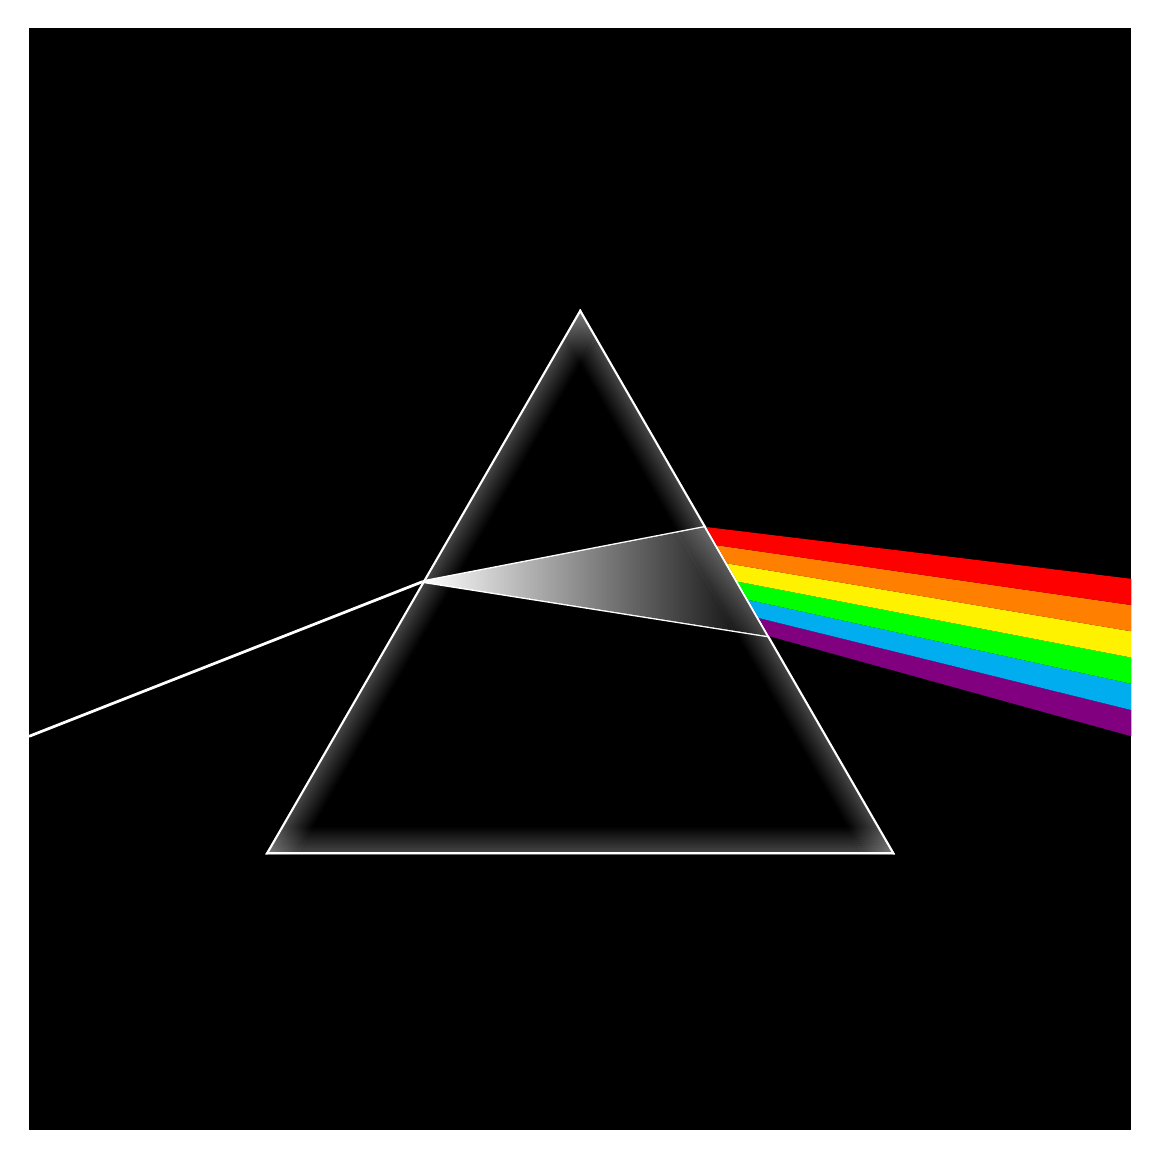
\begin{tikzpicture}	
	% Fill background
 	\fill[black] (0,0) rectangle (14,14);
 	
 	% Define coordinates
 	% source of light beam on the left side (S)
 	% prism vertices (P, Q, R)
 	% bottom and top of the diffused beam on the right side (B, T)
	\coordinate (S) at (0,5);
	\coordinate (P) at (3,3.5);
	\coordinate (Q) at (11,3.5);
	\coordinate (R) at (7,10.43);
	\coordinate (B) at (14,5);
	\coordinate (T) at (14,7);
	
	% mid point of the left prism edge (m)
	% bottom and top points where the diffused beam meets the right prism edge (b,t)
	\coordinate (m) at ($(R)!0.5!(P)$);
	\coordinate (b) at ($(Q)!0.4!(R)$);
	\coordinate (t) at ($(Q)!0.6!(R)$);
	
	% Draw light beam and shading
	\draw[white, line width=1pt] (S) -- (m);
	\draw[white, line width=1pt] (m) -- (t);
	\draw[white, line width=1pt] (m) -- (b);
	\shade[left color=white, right color=black] (m) -- (t) -- (b) -- cycle;

	\begin{scope}
	% Locally redefine colors in the code for rendering blur shadows (white to transparent and black to white)
	% https://github.com/norbusan/pgf-blur
	% cf. https://tex.stackexchange.com/questions/328433/elegant-way-to-modify-key-code-for-shadows-color
	\makeatletter
	\tikzset{render blur shadow/.code={
	    \pgfbs@savebb
	    \global\advance\pgfbs@fading@count by 1\relax
	    \pgfsyssoftpath@getcurrentpath{\pgfbs@input@path}%
	    \pgfbs@compute@shadow@bbox
	    \pgfbs@process@rounding{\pgfbs@input@path}{\pgfbs@fadepath}%
	    \pgfbs@apply@canvas@transform
	    \colorlet{pstb@shadow@color}{transparent!\pgfbs@opacity!white}%
	    \ifpgfbs@invert@fading
	    \pgfdeclarefading{shadowfading-\the\pgfbs@fading@count}{\pgfbs@paint@invert@fading}%
	    \else
	    \pgfdeclarefading{shadowfading-\the\pgfbs@fading@count}{\pgfbs@paint@fading}%
	    \fi
	    \pgfsetfillcolor{white}%
	    \pgfsetfading{shadowfading-\the\pgfbs@fading@count}%
	       {\pgftransformshift{\pgfpoint{\pgfbs@midx}{\pgfbs@midy}}}%
	    \pgfbs@usebbox{fill}%
	    \pgfbs@restorebb
	  },
	}
	\makeatother
	
	% Draw prism edges with shaded interior
	\clip (P) -- (Q) -- (R) -- cycle;
	\draw[white, line width=1.5pt, blur shadow={shadow xshift=0pt, shadow yshift=0pt, shadow blur steps=15, shadow blur radius=10pt}] (P) -- (Q);
	\draw[white, line width=1.5pt, blur shadow={shadow xshift=0pt, shadow yshift=0pt, shadow blur steps=15, shadow blur radius=10pt}] (Q) -- (R);
	\draw[white, line width=1.5pt, blur shadow={shadow xshift=0pt, shadow yshift=0pt, shadow blur steps=15, shadow blur radius=10pt}] (R) -- (P);
	\end{scope}
	
	% Split the bt and BT segments into 6 parts
	\foreach \i in {1,2,...,5} {
		\coordinate (p\i) at ($(b)!\i/6!(t)$);
		\coordinate (P\i) at ($(B)!\i/6!(T)$);
    }
    
    % Fill the various sections of the diffused beam with rainbow colors
	\fill[violet] (b) -- (B)  -- (P1) -- (p1) -- cycle;
	\fill[cyan] (p1) -- (P1)  -- (P2) -- (p2) -- cycle;
	\fill[green] (p2) -- (P2)  -- (P3) -- (p3) -- cycle;	
	\fill[yellow] (p3) -- (P3)  -- (P4) -- (p4) -- cycle;	
	\fill[orange] (p4) -- (P4)  -- (P5) -- (p5) -- cycle;	
	\fill[red] (p5) -- (P5)  -- (T) -- (t) -- cycle;
\end{tikzpicture}

\end{document}